\documentclass[letterpaper,journal,twoside]{IEEEtran}
\usepackage{amsmath,amsfonts}
\usepackage{array}
\usepackage{textcomp}
\usepackage{stfloats}
\usepackage{url}
\usepackage{verbatim}
\usepackage{graphicx}
\usepackage{cite}
\usepackage{xcolor}
\usepackage{subcaption}
\usepackage{mathtools}  
\usepackage{amssymb}
\usepackage{tabulary}
\usepackage{booktabs}
\usepackage[ruled,linesnumbered]{algorithm2e}
\usepackage{algorithmic}
\usepackage{hyperref}
\usepackage{setspace}

% usepackage from 
\usepackage{adjustbox}
\usepackage{physics}
\usepackage{amsmath}
\usepackage{tikz}
\usepackage{mathdots}
\usepackage{yhmath}
\usepackage{cancel}
\usepackage{color}
\usepackage{siunitx}
\usepackage{array}
\usepackage{multirow}
\usepackage{amssymb}
\usepackage{gensymb}
\usepackage{tabularx}
\usepackage{extarrows}
\usepackage{booktabs}
\usetikzlibrary{fadings}
\usetikzlibrary{patterns}
\usetikzlibrary{shadows.blur}
\usetikzlibrary{shapes}


\newcommand{\B}[1]{\mathbf{#1}}
\newcommand{\TB}[1]{\textbf{#1}}
\newcommand{\etal}{\textit{et al}.~}
\newcommand{\robotConfig}{\mathcal{C}}

\newcommand{\Norm}[1]{\lVert #1 \rVert}

\newcommand{\Btheta}{\boldsymbol{\theta}}
\newcommand{\Btau}{\boldsymbol{\tau}}
\newcommand{\Bomega}{\boldsymbol{\omega}}
\newcommand{\Beta}{\boldsymbol{\eta}}

\DeclareMathOperator*{\argmax}{arg\,max}
\DeclareMathOperator*{\argmin}{arg\,min}

\begin{document}

\title{Multi-drone Motion Planning \& Control in Dynamic Environment based on Deep Reinforcement Learning}

\author{
  \IEEEauthorblockN{
    Baozhe Zhang\textsuperscript{1} 
  }
}

\maketitle

\begingroup
\renewcommand\thefootnote{\textsuperscript{1}}
\footnotetext{School of Science and Engineering, 
The Chinese University of Hong Kong, Shenzhen, China. 
Email: \texttt{\{baozhezhang\}@link.cuhk.edu.cn}.
Baozhe Zhang is advised by Dr.~Tin Lun Lam and 
Dr.~Yuan Gao.}
\endgroup

% The paper headers
\markboth{ERG4901: Capstone Project -- Mid-Term Report}%
%{Shell \MakeLowercase{\textit{et al.}}: A Sample Article Using IEEEtran.cls for IEEE Journals}
{Zhang: Multi-drone Motion Planning \& Control}

% \IEEEpubid{\copyright~2023 Baozhe Zhang}
% Remember, if you use this you must call \IEEEpubidadjcol in the second
% column for its text to clear the IEEEpubid mark.


\begin{abstract}
TODO
\end{abstract}

\begin{IEEEkeywords}
  TODO
\end{IEEEkeywords}

\section{Introduction}
\IEEEPARstart{R}{ecently}, micro aerial vehicles (MAVs) or 
drones have been widely used in cinematography, search and 
rescue, inspection, and other tasks that require 
high-mobility or are difficult and unsafe for humans to 
operate. 
The planning and control system for plays a great role for 
unmanned aerial vehicles (UAVs) to perform the 
above mentioned tasks autonomously.

\section{Related Work}

In this section, we will investigate both traditional 
and RL-based methods for planning and control in the 
literature, with more focus on the aerial systems 
such as drones or quadrotors.
Traditional planning and control frameworks are decoupled.
% Path planning module serves as a frontend to find a geometric collision-free path in the given map, and motion planning module, based on the found path, finds the suitable dynamic-feasible motions for the robots. 
The path-(motion-)planning module serves as a guide system 
for the low-level controller driving the robot to move. 
This module needs to generate a geometrically 
collision-free and possibly kinodynamic feasible trajectory 
(or motion setpoints) for the low-level controller.
Then the low-level control module can use these motion 
setpoints to control the actuators on the robots to move.
Recent RL-based methods try to combine these two modules 
into a coupled system from repeated learning. 
The robots learn to navigate itself by trials and learning 
from the environments.
These trials are mostly conducted in simulations, 
where high-fidelity physics engines are required. 
By utilizing certain (deep) RL training methods, 
the trained models (e.g., neural networks) can be deployed 
on real robots for autonomous navigation in various static 
or dynamic environments.

\subsection{Configuration Space and Map Representation}
The configuration space (C-Space) contains all possible transformations
for robots. 
For a robot with $n$ degrees of freedom, the set of 
transformations, which is a manifold with dimension $n$, is 
the configuration space for that robot, denoted by $\robotConfig$
\cite{quan2020survey}. 
For example, the C-Space for the 2D rigid body is $SE(2)$ 
and for the 3D rigid body is $SE(3)$.
The obstacle region $\robotConfig_{\text{obs}} \subseteq \robotConfig$ 
is the transformations that the robot collide with the obstacles. 
The free space is defined as $\robotConfig_{\text{free}} = 
\robotConfig \backslash \robotConfig_{\text{obs}}$.
Therefore, the motion planning problem can be formulated as 
finding a path 
\begin{equation}
  \tau : \left[0,1\right]\rightarrow \robotConfig_{\text{free}}
\end{equation}
such that $\tau(0) = q_{\text{start}} 
\in \robotConfig_{\text{free}}$ and 
$\tau(1) = q_{\text{goal}} \in \robotConfig_{\text{free}}$
are the start and goal transformations, respectively.

Although mapping technique is usually coupled with the problem 
simultaneous localization and mapping (SLAM), mapping with
known pose of the robot is important as well. 
Many motion planning algorithms assume given maps, which means, 
in other words, the pose of the robot is known. 
One of the prevalent mapping representation is occupancy 
grid map \cite{elfes2013occupancy}, which divides the space
into cells (2D or 3D) storing the probabilistic estimate of the 
states (occupied or not).
Some data structure can be used to efficiently 
represent the space. 
The K-Dimensional Tree (K-D Tree) is an efficient data
structure that organizes multi-dimensional point data 
\cite{bentley1975multidimensional}
which enables fast search of nearest neighbors.
Incremental K-D Tree (ikd-tree) \cite{cai2021ikd} 
incrementally updates the K-D tree with only new points.
Octomap \cite{wurm2010octomap} based on octrees using 
probabilistic occupancy estimation proposes a compact 
data structure for map representation.
Another approach for volumetric representation is based on 
signed distance fields (SDFs) introduced in the computer
graphics literature \cite{curless1996volumetric}.
In recent robotic applications, \cite{lin2018autonomous} uses
truncated signed distance fields (TSDFs)
\footnote{The TSDF of a voxel is defined as the nearest 
distance to the surrounding surface in a truncation distance. 
If the voxel is between the robot and the surface, 
the value is positive, negative otherwise. }
to reconstruct the surfaces around the MAV. 
\cite{oleynikova2017voxblox} and later \cite{han2019fiesta}
use Euclidean signed distance fields (ESDFs) to incrementally
update the voxel map with distance and gradient information, 
which is convenient for gradient-based trajectory optimization.

\subsection{Traditional Planning and Control Methods}


\begin{figure}[h]
\center
\begin{adjustbox}{width=.5\textwidth}

\tikzset{every picture/.style={line width=0.75pt}} %set default line width to 0.75pt        

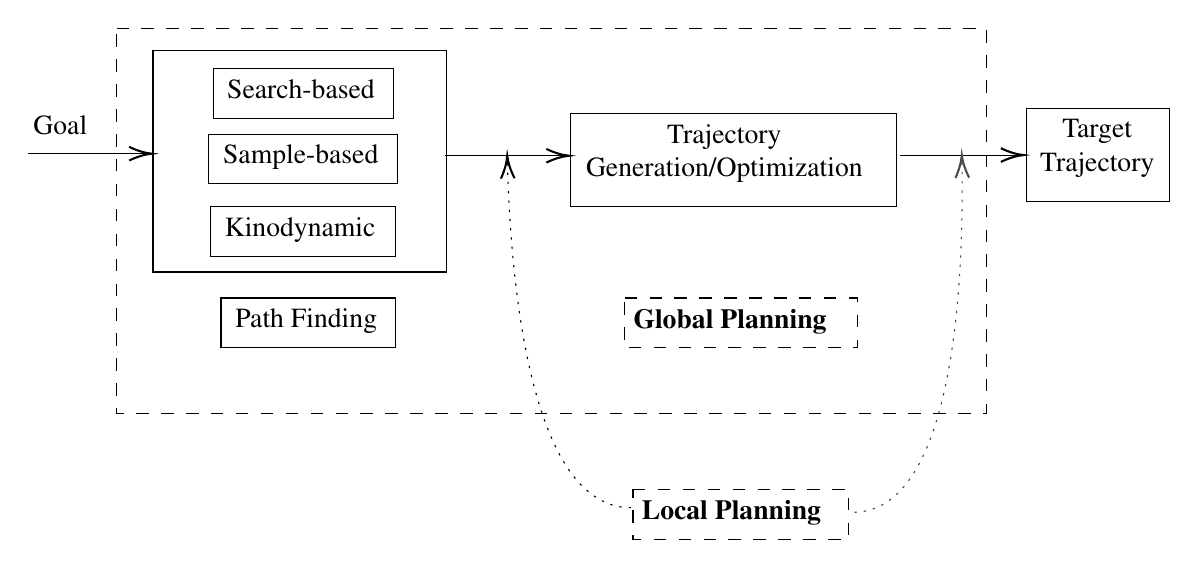
\begin{tikzpicture}[x=0.75pt,y=0.75pt,yscale=-1,xscale=1]
%uncomment if require: \path (0,267); %set diagram left start at 0, and has height of 267

%Shape: Rectangle [id:dp575866165243341] 
\draw   (89.56,19.67) -- (230.89,19.67) -- (230.89,126.44) -- (89.56,126.44) -- cycle ;
%Straight Lines [id:da8414235785777104] 
\draw    (230.44,70.44) -- (288,70.44) ;
\draw [shift={(290,70.44)}, rotate = 180] [color={rgb, 255:red, 0; green, 0; blue, 0 }  ][line width=0.75]    (10.93,-3.29) .. controls (6.95,-1.4) and (3.31,-0.3) .. (0,0) .. controls (3.31,0.3) and (6.95,1.4) .. (10.93,3.29)   ;
%Straight Lines [id:da08815651015896142] 
\draw    (29.44,69.44) -- (87,69.44) ;
\draw [shift={(89,69.44)}, rotate = 180] [color={rgb, 255:red, 0; green, 0; blue, 0 }  ][line width=0.75]    (10.93,-3.29) .. controls (6.95,-1.4) and (3.31,-0.3) .. (0,0) .. controls (3.31,0.3) and (6.95,1.4) .. (10.93,3.29)   ;
%Straight Lines [id:da22108099082080424] 
\draw    (449.44,70.11) -- (507,70.11) ;
\draw [shift={(509,70.11)}, rotate = 180] [color={rgb, 255:red, 0; green, 0; blue, 0 }  ][line width=0.75]    (10.93,-3.29) .. controls (6.95,-1.4) and (3.31,-0.3) .. (0,0) .. controls (3.31,0.3) and (6.95,1.4) .. (10.93,3.29)   ;
%Curve Lines [id:da017803972324741846] 
\draw [color={rgb, 255:red, 0; green, 0; blue, 0 }  ,draw opacity=1 ] [dash pattern={on 0.84pt off 2.51pt}]  (319.78,240) .. controls (270.94,240) and (261.74,130.66) .. (260.26,72.2) ;
\draw [shift={(260.22,70.44)}, rotate = 88.68] [color={rgb, 255:red, 0; green, 0; blue, 0 }  ,draw opacity=1 ][line width=0.75]    (10.93,-3.29) .. controls (6.95,-1.4) and (3.31,-0.3) .. (0,0) .. controls (3.31,0.3) and (6.95,1.4) .. (10.93,3.29)   ;
%Curve Lines [id:da912860022154641] 
\draw [color={rgb, 255:red, 74; green, 74; blue, 74 }  ,draw opacity=1 ] [dash pattern={on 0.84pt off 2.51pt}]  (427.56,242.22) .. controls (475.74,240.9) and (480.46,130.36) .. (479.26,71.87) ;
\draw [shift={(479.22,70.11)}, rotate = 88.68] [color={rgb, 255:red, 74; green, 74; blue, 74 }  ,draw opacity=1 ][line width=0.75]    (10.93,-3.29) .. controls (6.95,-1.4) and (3.31,-0.3) .. (0,0) .. controls (3.31,0.3) and (6.95,1.4) .. (10.93,3.29)   ;
%Shape: Rectangle [id:dp5818665047698117] 
\draw  [dash pattern={on 4.5pt off 4.5pt}] (72,9) -- (491,9) -- (491,194.5) -- (72,194.5) -- cycle ;

% Text Node
\draw    (122.33,139) -- (206.33,139) -- (206.33,163) -- (122.33,163) -- cycle  ;
\draw (125.33,143) node [anchor=north west][inner sep=0.75pt]   [align=left] {\begin{minipage}[lt]{55.15pt}\setlength\topsep{0pt}
\begin{center}
{\fontfamily{ptm}\selectfont Path Finding}
\end{center}

\end{minipage}};
% Text Node
\draw    (118.5,28.5) -- (205.5,28.5) -- (205.5,52.5) -- (118.5,52.5) -- cycle  ;
\draw (121.5,32.5) node [anchor=north west][inner sep=0.75pt]   [align=left] {\begin{minipage}[lt]{57.1pt}\setlength\topsep{0pt}
\begin{center}
{\fontfamily{ptm}\selectfont Search-based}
\end{center}

\end{minipage}};
% Text Node
\draw    (116.5,60) -- (207.5,60) -- (207.5,84) -- (116.5,84) -- cycle  ;
\draw (119.5,64) node [anchor=north west][inner sep=0.75pt]   [align=left] {\begin{minipage}[lt]{59.94pt}\setlength\topsep{0pt}
\begin{center}
{\fontfamily{ptm}\selectfont Sample-based}
\end{center}

\end{minipage}};
% Text Node
\draw    (117.33,95) -- (206.33,95) -- (206.33,119) -- (117.33,119) -- cycle  ;
\draw (120.33,99) node [anchor=north west][inner sep=0.75pt]   [align=left] {\begin{minipage}[lt]{58.25pt}\setlength\topsep{0pt}
\begin{center}
{\fontfamily{ptm}\selectfont Kinodynamic}
\end{center}

\end{minipage}};
% Text Node
\draw    (290.78,50) -- (447.78,50) -- (447.78,95) -- (290.78,95) -- cycle  ;
\draw (293.78,54) node [anchor=north west][inner sep=0.75pt]   [align=left] {\begin{minipage}[lt]{104.69pt}\setlength\topsep{0pt}
\begin{center}
{\fontfamily{ptm}\selectfont Trajectory }\\{\fontfamily{ptm}\selectfont Generation/Optimization}
\end{center}

\end{minipage}};
% Text Node
\draw (30.67,49.67) node [anchor=north west][inner sep=0.75pt]   [align=left] {{\fontfamily{ptm}\selectfont Goal}};
% Text Node
\draw    (510.33,47.67) -- (579.33,47.67) -- (579.33,92.67) -- (510.33,92.67) -- cycle  ;
\draw (513.33,51.67) node [anchor=north west][inner sep=0.75pt]   [align=left] {\begin{minipage}[lt]{44.84pt}\setlength\topsep{0pt}
\begin{center}
{\fontfamily{ptm}\selectfont Target }\\{\fontfamily{ptm}\selectfont Trajectory}
\end{center}

\end{minipage}};
% Text Node
\draw  [dash pattern={on 4.5pt off 4.5pt}]  (320.8,231.22) -- (424.8,231.22) -- (424.8,255.22) -- (320.8,255.22) -- cycle  ;
\draw (323.8,235.22) node [anchor=north west][inner sep=0.75pt]   [align=left] {{\fontfamily{ptm}\selectfont \textbf{Local Planning}}};
% Text Node
\draw  [dash pattern={on 4.5pt off 4.5pt}]  (316.8,139) -- (428.8,139) -- (428.8,163) -- (316.8,163) -- cycle  ;
\draw (319.8,143) node [anchor=north west][inner sep=0.75pt]   [align=left] {{\fontfamily{ptm}\selectfont \textbf{Global Planning}}};


\end{tikzpicture}
\end{adjustbox}
\caption{Traditional planning pipeline.}
\label{fig:concept}
\end{figure}

In general, path-planning algorithms for robot navigation 
can be divided into two major categories: 
global and local methods.
\footnote{The reader should note that there is no strict 
line between global and local planning methods, since
it can also be argued that with high-frequency global
re-planning, local path planning can be avoided.}  
Global methods focus on finding collision-free paths from 
the current robot position to a global goal position mostly 
in static scenes, while local methods tend to reactively 
avoid both static and dynamic obstacles. 
In order to generate smooth trajectories for robots to 
follow, based on the discrete planned waypoints, the 
trajectory optimization module is usually added in the 
whole pipeline. 
Usually in the literature, the path-finding module 
is called the frontend and the 
trajectory-optimization module is called the backend. 
A typical traditional planning pipeline can be 
found in Fig.~\ref{fig:concept}.

\subsubsection{Path finding (frontend)}

In the path-finding stage of the global planning, 
the methods can be categorized 
from three major directions: \TB{search-based}, 
\TB{sample-based}, and \TB{kinodynamic} methods. 


% \begin{algorithm}
\caption{A* Algorithm}
\label{alg:a_star}
\begin{algorithmic}[1]
\REQUIRE $start$: starting node, $goal$: goal node
\STATE $openSet \gets \{start\}$
\STATE $cameFrom \gets$ empty map
\STATE $gScore[start] \gets 0$
\STATE $fScore[start] \gets heuristic(start, goal)$
\WHILE{$openSet$ is not empty}
  \STATE $current \gets$ node in $openSet$ with lowest $fScore$
  \IF{$current = goal$}
    \RETURN reconstructPath($cameFrom$, $current$)
  \ENDIF
  \STATE remove $current$ from $openSet$
  \FORALL{$neighbor$ of $current$}
    \STATE $tentativeGScore \gets gScore[current] + dist(current, neighbor)$
    \IF{$neighbor$ not in $gScore$ or $tentativeGScore < gScore[neighbor]$}
      \STATE $cameFrom[neighbor] \gets current$
      \STATE $gScore[neighbor] \gets tentativeGScore$
      \STATE $fScore[neighbor] \gets gScore[neighbor] + heuristic(neighbor, goal)$
      \IF{$neighbor$ not in $openSet$}
        \STATE add $neighbor$ to $openSet$
      \ENDIF
    \ENDIF
  \ENDFOR
\ENDWHILE
\RETURN failure
\end{algorithmic}
\end{algorithm}

\TB{Search-based} algorithms such as depth-first 
search (DFS) \cite{cormen2022introduction}, 
breadth-first search (BFS) \cite{cormen2022introduction}, 
Dijkstra \cite{wang2011application}, and 
A* \cite{hart1968formal}, use graph-search methods 
possibly with certain pre-defined heuristics to find 
geometrically feasible paths on given grid maps. 
A key assumption for these methods to perform path-finding 
is the map is given, which can be difficult to be obtained 
in certain situations. 
Though these search-based methods can perform well, they 
can have longer search time when the space scales.
% Alg.~\ref{alg:a_star} shows the A* path-planning algorithm which returns the shortest path from the source node to the target node. 
\TB{Sample-based} methods such as rapidly exploring random 
tree (RRT), probabilistic roadmap (PRM), and their 
variants (e.g., RRT* and PRM*) use sampling in C-Space. 
to crate collision-free paths \cite{lavalle2001rapidly,
karaman2011sampling,kavraki1996probabilistic}. 
The general form of RRT algorithm can be found in 
Alg.~\ref{alg:rrt}.
\begin{algorithm}
\SetAlgoLined
\KwIn{Start state $q_{start}$, goal region $G$, maximum number of iterations $K$, step size $\Delta q$, collision checking function $IsCollisionFree$, tree $T$}
\KwOut{A path from $q_{start}$ to $G$ if found, otherwise failure}
Add $q_{start}$ to $T$\;
\For{$k=1$ \KwTo $K$}{
  $q_{rand} \gets$ RandomState()\;
  $q_{near} \gets$ NearestVertex($T$, $q_{rand}$)\;
  $q_{new} \gets$ Steer($q_{near}$, $q_{rand}$, $\Delta q$)\;
  \If{!IsCollisionFree($q_{near}$, $q_{new}$)}{
    continue\;
  }
  Add $q_{new}$ to $T$\;
  \If{$q_{new} \in G$}{
    \Return Path($q_{start}$, $q_{new}$)\;
  }
}
\Return failure\;
\caption{Rapidly-Exploring Random Tree (RRT)}
\label{alg:rrt}
\end{algorithm}

However, the tree nodes in these methods need to cover the 
whole C-Space which may suffer from heavy computational 
loads especially when the space is large.  

Both search- and sample-based methods can generate 
geometrically collision-free paths but possibly jerky
\footnote{Jerk $\B{j}$ is the third time-derivative 
of the position $\B{p}$} or 
violating the underlying robots' dynamics.
For example, most ground vehicles are not 
holonomic, i.e., they cannot move freely in all directions 
in 2D space, where their motions are governed by their 
mechanical and motion constraints (e.g., velocities and 
accelerations).
In order to obey both the kinematic and dynamic 
constraints for specific
robot platforms and reduce the stress of the backend 
optimization part, \TB{kinodynamic} methods are introduced
in the literature. 
Donald \etal \cite{donald1993kinodynamic} first proposed 
the term \TB{kinodynamic} motion planning in the literature.
The authors proposed the first provably good approximation 
algorithm about the motion planning for a point-mass model 
in 2D and 3D environments with polyhedral obstacles.
State-lattice method \cite{pivtoraiko2011kinodynamic} is also 
used for kinodynamic motion 
planning, where the boundary value problem (BVP) needs to be 
solved to get the corresponding control inputs 
for the sampled states. 
In \cite{zhou2019robust}, the authors propose a method 
sampling in the control space to generate possible motion 
primitives and then 
based on these motions search and select kinodynamic 
feasible paths. 
Webb and Berg \cite{webb2013kinodynamic} propose the method
kinodynamic RRT* generalizing the
earlier work on RRT* \cite{karaman2011sampling} for kinodynamic 
systems, as it guarantees asymptotic optimality for 
any system with controllable linear
dynamics, in state spaces of any dimension.
\cite{dolgov2008practical,dolgov2009autonomous,dolgov2010path}
propose the algorithm hybrid A* (or hybrid-state A*) extending 
original A* algorithm for kinodynamic graph searching.

Other less common method such as model predictive 
control (MPC) added with obstacle constraints or with 
additional environment-related 
terms \cite{park2009obstacle,ji2016path}  can also be 
used to generate collision-free paths, which is based on 
quadratic-programming (QP) optimization. 
However, MPC-related methods need to tradeoff among the 
length of the time horizon, the computational loads, and 
optimality. Short time horizon often leads the problem to 
sub-optimal solutions.




\subsubsection{Trajectory generation and optimization (backend)}
Most path-finding algorithms only generate geometric 
feasible paths, without any time information. 
The goal for trajectory generation and optimization is to 
provide both spatial and temporal profiles based on the 
found paths \cite{quan2020survey}. 
In essential, the trajectory is a geometric path parametrized 
in time, with guaranteed kinodynamic feasibility and smoothness.
Usually, it is optimized with goals such as minimizing the 
total ``energy'' spent along the path while satisfying the 
kinodynamic constraints of the robots.
Mellinger and Kumar \cite{mellinger2011minimum} propose 
a minimum snap trajectory generation method based on the 
differential flat property of the quadrotor or multirotor 
systems. 
This method uses quadratic-programming (QP) optimization with 
hard constraints for flight corridors to generate optimal 
trajectories. 
In the literature, one of the prevalent methods is 
interpolating curves \cite{dong2023review}.
Zhou \etal \cite{zhou2019robust} propose a trajectory 
optimization method based on the convex hull property of 
B-splines and provide a time adjustment method for it.
Wang \etal \cite{wang2022geometrically} propose a 
minimum-control (MINCO) trajectory family based on 
multi-degree polynomials that can be 
optimized with user-defined state-input constraints for 
multi-copter motion planning.
Gradient-based methods such as
CHOMP \cite{ratliff2009chomp} and 
EGO-Planner \cite{zhou2020ego} are also popular methods 
for trajectory optimization.

\subsubsection{Local methods}
Most global methods perform well in static environments, 
but poorly in dynamic environments. 
Local path-planning methods can be employed to handle 
this problem. 
An early local obstacle-avoidance method is artificial 
potential field (APF) \cite{warren1989global}.
APF formulates the potentials on a given path as the 
inside and outside ones, and pushes the path from 
high-potential to low-potential region by finding the 
lowest potential value. 
If the waypoints on the path across the 
obstacle (in the obstacle), the potential is formulated as 
\begin{equation}
\label{eq:APF_in}
U_{\text{in}} = 
U_{\text{max}}(1 - \frac{R_{\text{in}}}{R_{\text{max}}}) + 
U_{\text{offset}}
\end{equation}
where $U_{\text{max}}$ is the max potential, 
$R_{\text{in}}$ is the distance to the centroid of the 
obstacle, $R_{\text{max}}$ is the max radius of the 
obstacle, and $U_{\text{offset}}$ is the extra 
potential penalty.
The outside potential is formulated as 
\begin{equation}
\label{eq:APF_out}
U_{\text{out}} = 
\frac{1}{2}U_{\text{offset}}(1+ \frac{1}{1+R_\text{out}})
\end{equation}
where $R_{\text{out}}$ is the distance outside the obstacle.
APF can be used for quadrotor path-planning \cite{chen2016uav}.
However, when multiple obstacles presented, APF can suffer 
from the problem of local minimum \cite{koren1991potential}.
Dynamic window approach (DWA) \cite{seder2007dynamic} can 
be used for dynamic obstacle avoidance, where DWA considers
the kinodynamic feasibility of the robot and samples in the 
velocity space to generate motion primitives for collision 
avoidance. 
The idea of velocity obstacle (VO) is proposed and generalized
by Van Den Berg \cite{van2011reciprocal,van2011reciprocal2,bareiss2013reciprocal}.
Reciprocal VO-based obstacle avoidance methods can be used for
for motion planning for robots.  
However, the smoothness of the generated paths cannot be 
guaranteed. 
Dynamical system modulation (DSM)
\cite{khansari2012dynamical,huber2022fast,huber2023avoidance}
is another approach to achieve obstacle avoidance for local
motion planning, which directly changes the first-order 
linear system of the robot (point-mass model) to guide the 
robot away from the obstacle by adding a linear transformation
(obtained from the environments) to the initial velocity of 
the robot.
However, the algorithms are limited with star-shaped obstacles, 
and the performance of DSM on agile robots such as quadrotors
is still skeptical.

\subsubsection{Control}
The control module is usually responsible for trajectory 
tracking (TT) tasks for planning and control.
Despite the low-level controllers of the actuators of the 
robots, which track the setpoints of torques, angular 
velocities, or accelerations, the controllers used in TT
phase focus on designing controllers based on system
equations so that robots can track a given reference 
trajectory asymptotically. 
\cite{majd2019stable} proposes using the input-output 
linearization technique to optimize the tracking error for
car-like robot trajectory tracking.
Model predictive control (MPC) or receding horizon control (RHC)
is also a popular method to perform TT via optimization.
\cite{kunhe2005mobile} used non-linear MPC to control the 
wheeled robots for TT.
\cite{romero2022model,ji2021cmpcc} propose model predictive
contouring control (MPCC) by adding the time profile to the 
controller design to minimize the traversal time while tracking
the reference trajectory.
Thanks to the flexibility of the framework of MPC, the model 
can be reformulated to satisfy different needs. 
In \cite{zhang2023coni}, the authors propose cooperative 
non-inertial frame based model predictive control (CoNi-MPC), 
which directly formulates the quadrotor model in a target's 
body non-inertial frame and controls the quadrotor tracking 
trajectories pre-defined in the target's frame.

\subsection{RL-based Planning and Control}

\subsection{Multi-robot Planning and Control}

\section{Problem Formulation}

\bibliographystyle{IEEEtran}
\bibliography{report}


\end{document}


